\documentclass[10pt]{beamer}

\usetheme{metropolis}
\usepackage{appendixnumberbeamer}

\usepackage{booktabs}
\usepackage[scale=2]{ccicons}

\usepackage{pgfplots}
\usepgfplotslibrary{dateplot}

\usepackage{xspace}
\newcommand{\themename}{\textbf{\textsc{metropolis}}\xspace}

\newcommand{\norm}[1]{\left\lVert#1\right\rVert}

% %%%%%%%%%%%%%%%%%%%%%%%%%%%%%%%%%%%%%%%%%%%%%%%%%%%%%%%%%%%%%%%%%%%%%%%%%%%%%

\title{SVM Algorithm}
\subtitle{based on Lagrangian multipliers and KKT conditions}
\date{\today}
\author{Matteo Conti}
\institute{University of Bologna}
% \titlegraphic{\hfill\includegraphics[height=1.5cm]{logo.pdf}}

% % % % % % % % % % % % % % % % % % % % % % % % % % % % % % % % % % % % % % % %

\begin{document}

\maketitle

\begin{frame}{Table of contents}
  \setbeamertemplate{section in toc}[sections numbered]
  \tableofcontents[hideallsubsections]
\end{frame}

% %%%%%%%%%%%%%%%%%%%%%%%%%%%%%%%%%%%%%%%%%%%%%%%%%%%%%%%%%%%%%%%%%%%%%%%%%%%%%

\section{Problem Formulation}
\begin{frame}[fragile]{Our Problem}
  \begin{columns}[onlytextwidth, T, c]
    \begin{column}{.5\textwidth}
      initial constrainted problem:
      \newline
      \begin{equation*}
        \begin{split}
          \text{min}\ &\ \frac{1}{2} \norm{w}^2 \\
          \text{s.t.}\ &\ \forall_{i}\ y_i (x_i \cdot w + b) -1 \geq 0
        \end{split}
      \end{equation*}
    \end{column}
    \begin{column}{.5\textwidth}
        \begin{figure}
          \centering    
          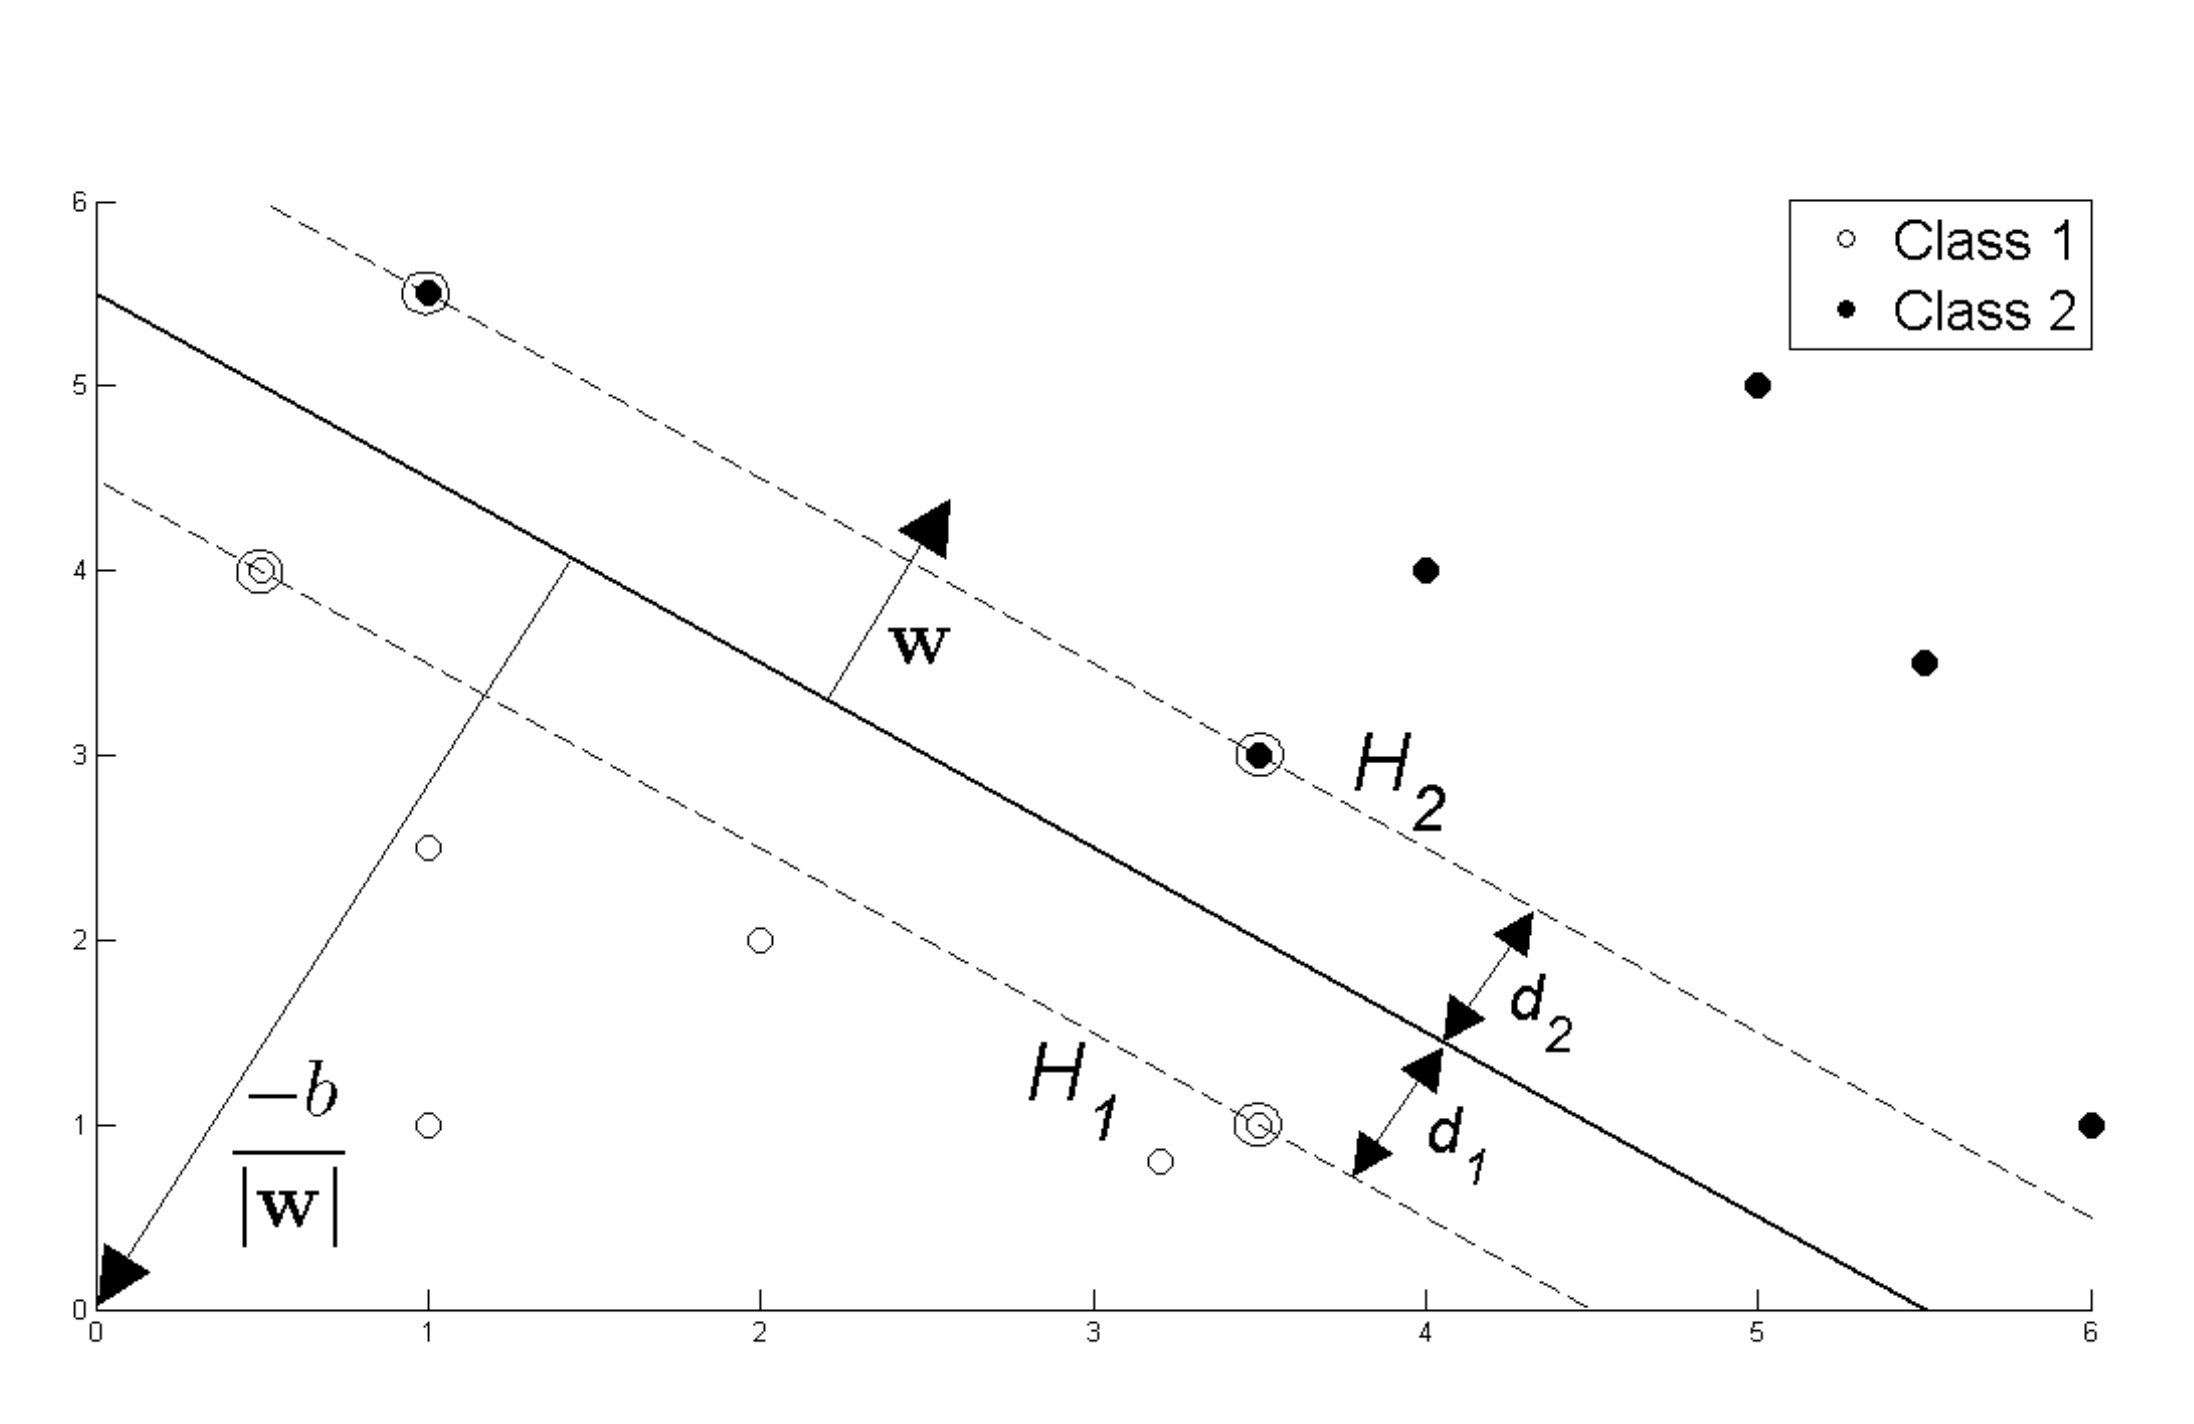
\includegraphics[width=5cm]{assets/images/s1.01.png}
        \end{figure}
    \end{column}    
  \end{columns}
  
  \vspace{.7cm}
  
  % where the hyperplane equation is $w \cdot x + b = 0$
  % and the perpendicular distance from the hyperplane to the origin is $\frac{b}{\norm{w}}$
  the points (circled) $H1$ and $H2$ that lie closest to the separating hyperplane, 
  i.e. the \textbf{Support Vectors}, can be described by
  \begin{equation*}
    \begin{split}
      x_i \cdot w + b = +1 & \hspace{.5cm} \text{for} \hspace{.5cm} H1 \\
      x_i \cdot w + b = -1 & \hspace{.5cm} \text{for} \hspace{.5cm} H2
    \end{split}
  \end{equation*}

\end{frame}


\begin{frame}[fragile]{Lagrangian Multipliers Strategy}
  we formulate our problem as:
  \newline
  \begin{equation*}
    \begin{split}
      L_P\ \equiv\ \frac{1}{2} \norm{w}^2 - \alpha [\forall_i\  y_i (x_i \cdot w + b) - 1]
    \end{split}
  \end{equation*}

  where $\alpha_i$ are the Lagrange \textbf{multipliers} such that:
  \begin{equation*}
    \forall_i\ \alpha_i\ \geq 0 
  \end{equation*}

  we want to \textbf{min} $L_P(w,b)$ and then \textbf{max} $L_P(\alpha)$.
\end{frame}


\begin{frame}[fragile]{Final Problem Formulation}
  Dual form of the primary Lagrangian problem:
  \newline
  \begin{equation*}
    \begin{split}
      \max_{\alpha}\ &\ L_D\ \equiv\ \sum_{i=1}^{L} \alpha_i - \frac{1}{2} \sum_{i,j} \alpha_i \alpha_j y_i y_j x_i \cdot x_j
      \equiv\ \sum_{i=1}^{L} \alpha_i - \frac{1}{2} \alpha^T H \alpha
    \end{split}
  \end{equation*}

  where:
  \newline
  \begin{equation*}
    H\ \equiv\ y_i y_j x_i \cdot x_j
  \end{equation*}

  subject to:
  \newline
  \begin{equation*}
    \sum_{i=1}^{L} \alpha_i y_i = 0 \hspace{.5cm} \text{and} 
    \hspace{.5cm} 
    \forall_i\ \alpha_i \geq 0 
  \end{equation*}
\end{frame}


% % % % % % % % % % % % % % % % % % % % % % % % % % % % % % % % % % % % % % % %

\section{Quadratic-Programming Optimization}
\begin{frame}[fragile]{Quadratic-Programming Solver}
  We have used the \emph{cvxopt} Python library in order to obtain the 
  solutions for our Quadratic-Programming problem.
  \vspace{.5cm}

  This library solve a problem in the form
  \begin{equation*}
    \begin{split}
      \min_{x}\ &\ \ \frac{1}{2} x^T P x + q^T x \\
          s.t.\ &\ \ Gx \leq h \\
              \ &\ \ Ax = b
    \end{split}
  \end{equation*}
  \vspace{.5cm}

  So we've ended up in adapting our $max_{x}\ L_D$ problem to the above formulation
  in order to find $\alpha_i$ solutions (look at the code for more details).
\end{frame}


% % % % % % % % % % % % % % % % % % % % % % % % % % % % % % % % % % % % % % % %

\section{Soft-Margin Assumption}
\begin{frame}[fragile]{Soft-Margin Assumption}
  \textcolor{lightgray}{Dual form of the primary Lagrangian problem:}
  \newline
  \begin{equation*}
    \begin{split}
      \textcolor{lightgray}{\max_{\alpha}\ \sum_{i=1}^{L} \alpha_i - \frac{1}{2} \alpha^T H \alpha}
    \end{split}
  \end{equation*}

  subject to:
  \newline
  \begin{equation*}
    \textcolor{lightgray}{\sum_{i=1}^{L} \alpha_i y_i = 0 \hspace{.5cm} \text{and}}
    \hspace{.5cm} 
    \textcolor{blue}{\forall_i\ \mathbf{C \geq \alpha_i \geq 0}}
  \end{equation*}

  \vspace{.3cm}

  where $\mathbf{C}$ controls the trade-off between the slack variable penalty 
  and the size of the margin (a low $\mathbf{C}$ makes the hyperplane decision 
  surface smooth, while a high $\mathbf{C}$ aims at classifying all points correctly).
\end{frame}

\begin{frame}[fragile]{Hard-Margin vs Soft-Margin}
  \begin{columns}[onlytextwidth, T, c]
    \begin{column}{.5\textwidth}
        \begin{figure}
            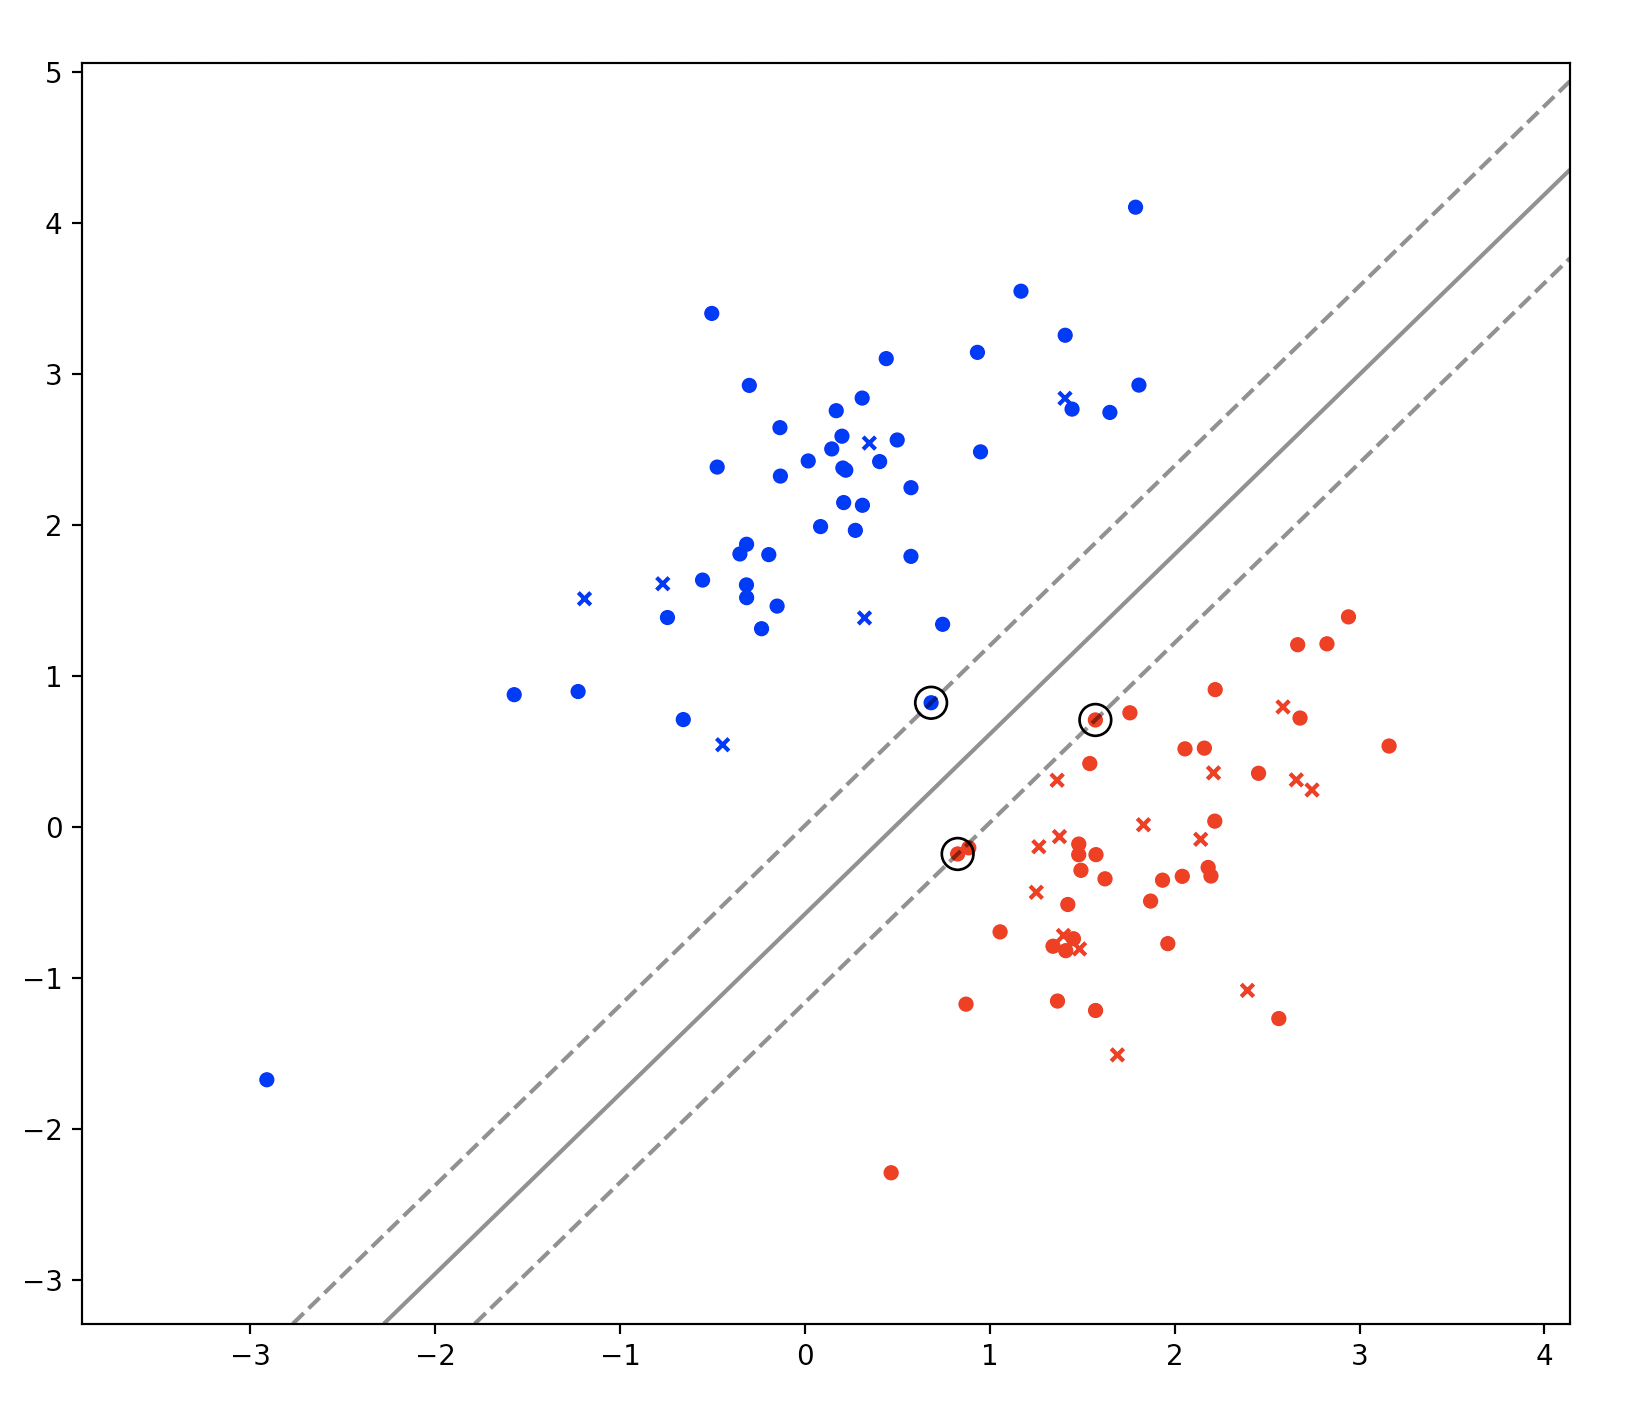
\includegraphics[width=5cm]{assets/images/s3.01.png}
            \caption{Hard-Margin}
        \end{figure}
    \end{column}
    \begin{column}{.5\textwidth}
        \begin{figure}
            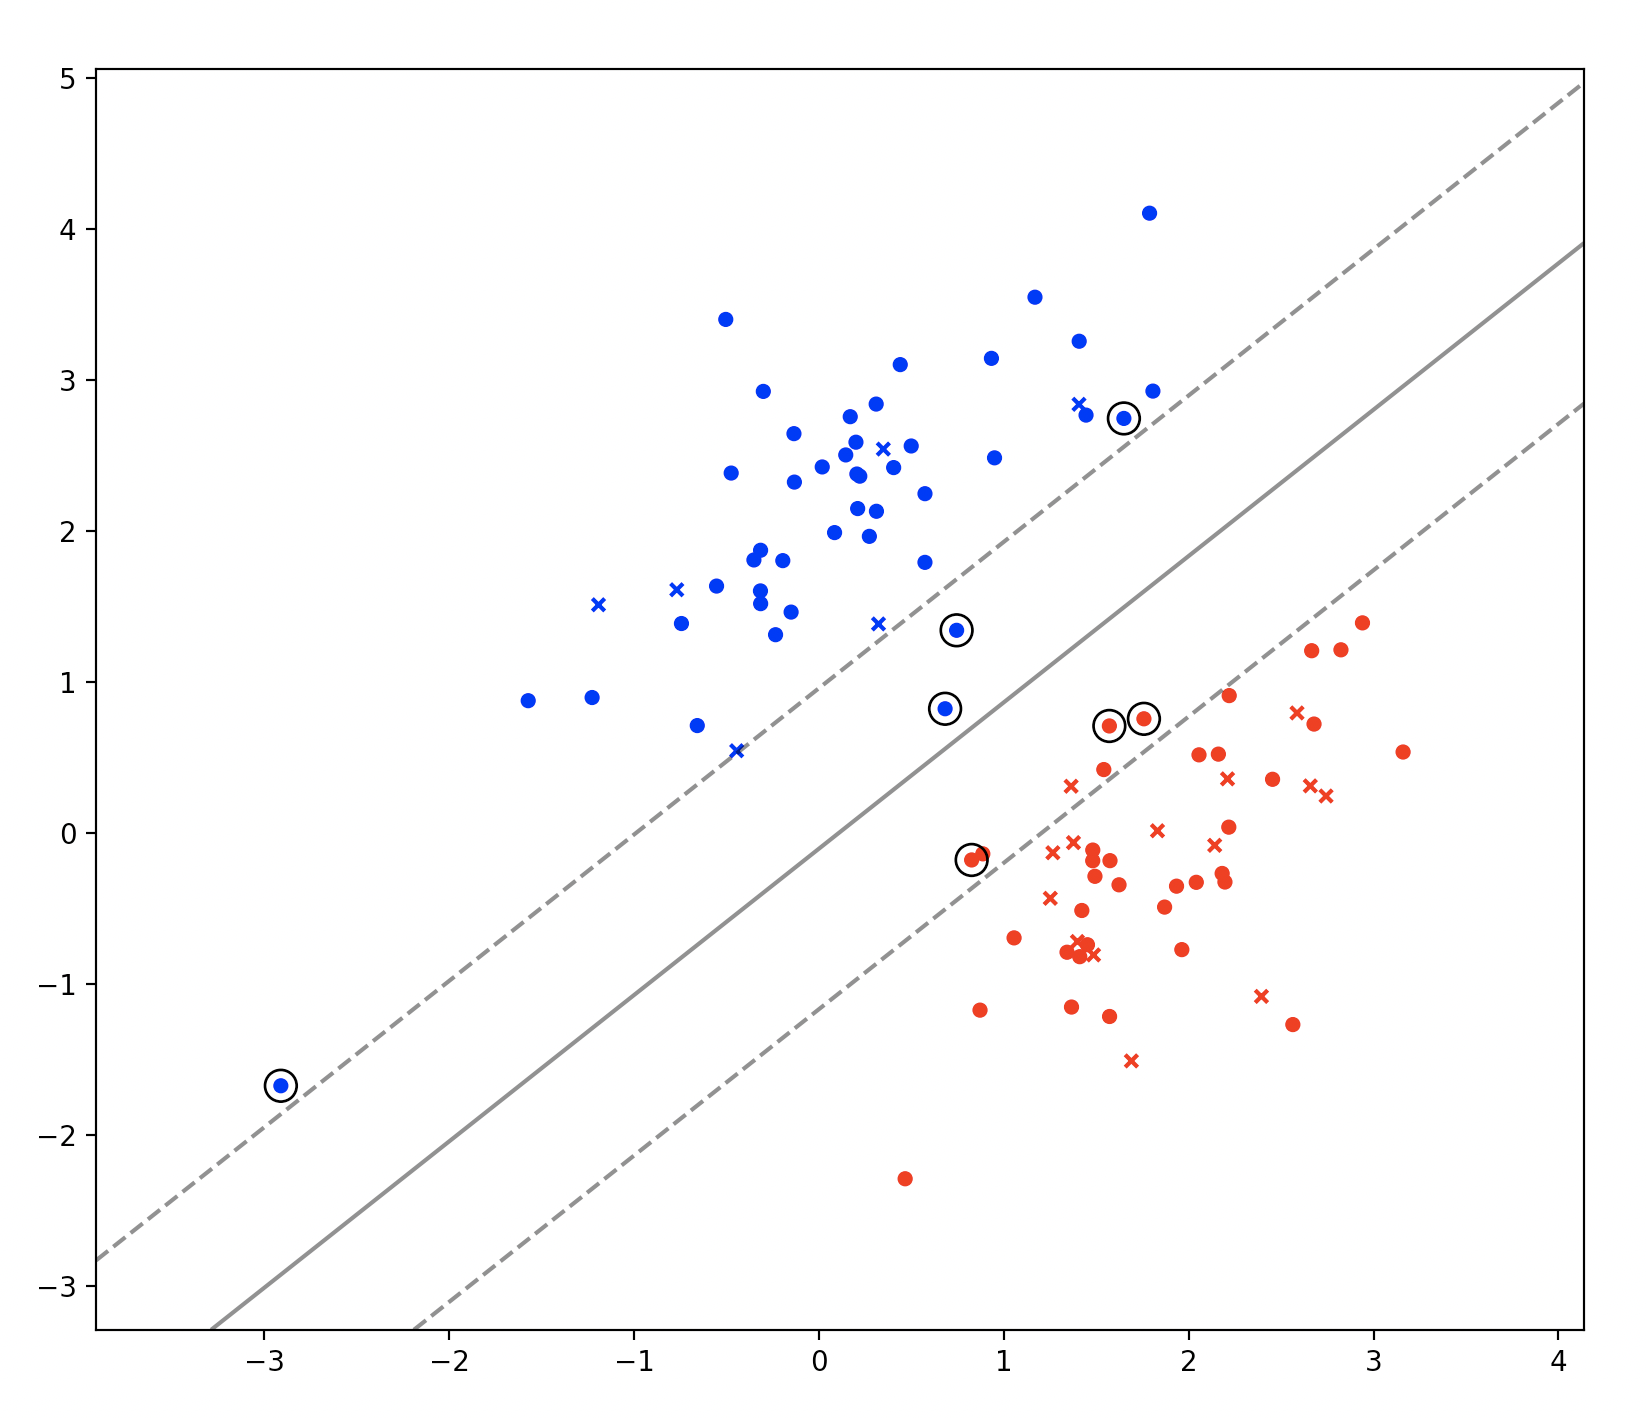
\includegraphics[width=5cm]{assets/images/s3.02.png}
            \caption{Soft-Margin}
        \end{figure}
    \end{column}    
  \end{columns}
\end{frame}


% % % % % % % % % % % % % % % % % % % % % % % % % % % % % % % % % % % % % % % %

\section{Non-Linear Kernel}
\begin{frame}[fragile]{Non-Linear Kernel}
  Dual form of the primary Lagrangian problem:
  \newline
  \begin{equation*}
    \begin{split}
      \textcolor{blue}{\max_{\alpha}}\ &\ \textcolor{blue}{L_D}\ 
      \equiv\ 
      \textcolor{lightgray}{\sum_{i=1}^{L} \alpha_i - \frac{1}{2} \alpha^T} 
      \mathbf{\textcolor{blue}{H}}
      \textcolor{lightgray}{\alpha}
    \end{split}
  \end{equation*}

  where:
  \newline
  \begin{equation*}
    \textcolor{blue}{H}\ \equiv\ \textcolor{lightgray}{y_i y_j} \mathbf{\textcolor{blue}{k(x_i, x_j)}}
  \end{equation*}

  linear kernel is defined as:
  \begin{equation*}
    k(x_i, x_j) = \phi(x_i) \cdot \phi(x_j)
  \end{equation*}

  polynomial kernel is defined as:
  \begin{equation*}
    k(x_i, x_j) = (\phi(x_i) \cdot \phi(x_j) + 1)^{deg}
  \end{equation*}
\end{frame}

\begin{frame}[fragile]{Non-Linear Kernel}
  \begin{columns}[onlytextwidth, T, c]
    \begin{column}{.5\textwidth}
        \begin{figure}
            % TODO: ...
            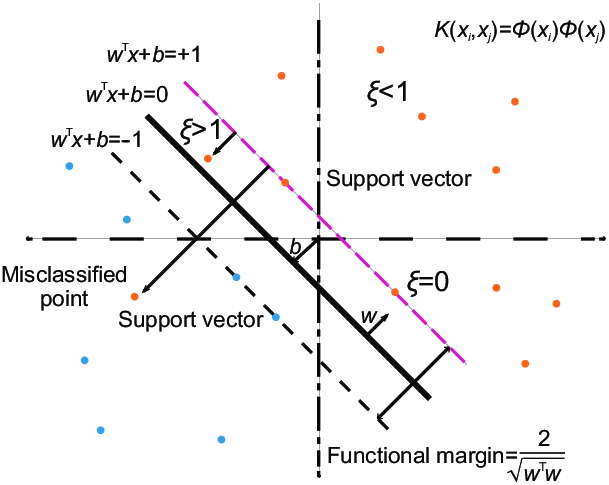
\includegraphics[width=5cm]{assets/images/test.png}
            \caption{Linear Kernel}
        \end{figure}
    \end{column}
    \begin{column}{.5\textwidth}
        \begin{figure}
            % TODO: ...
            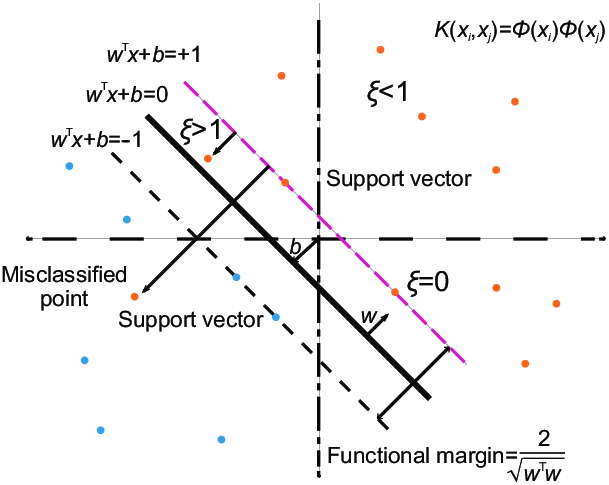
\includegraphics[width=5cm]{assets/images/test.png}
            \caption{Polynomial Kernel}
        \end{figure}
    \end{column}    
  \end{columns}
\end{frame}


% % % % % % % % % % % % % % % % % % % % % % % % % % % % % % % % % % % % % % % %

\begin{frame}[standout]
  \small{
    \emph{https://github.com/contimatteo/SVM-from-scratch}
  }
\end{frame}

% % % % % % % % % % % % % % % % % % % % % % % % % % % % % % % % % % % % % % % %

% \section{Title formats}

% \begin{frame}{Metropolis title formats}
% 	\themename supports 4 different title formats:
% 	\begin{itemize}
% 		\item Regular
% 		\item \textsc{Small caps}
% 		\item \textsc{all small caps}
% 		\item ALL CAPS
% 	\end{itemize}
% 	They can either be set at once for every title type or individually.
% \end{frame}

% {
%     \metroset{titleformat frame=smallcaps}
% \begin{frame}{Small caps}
% 	This frame uses the \texttt{smallcaps} title format.

% 	\begin{alertblock}{Potential Problems}
% 		Be aware that not every font supports small caps. If for example you typeset your presentation with pdfTeX and the Computer Modern Sans Serif font, every text in small caps will be typeset with the Computer Modern Serif font instead.
% 	\end{alertblock}
% \end{frame}
% }

% {
% \metroset{titleformat frame=allsmallcaps}
% \begin{frame}{All small caps}
% 	This frame uses the \texttt{allsmallcaps} title format.

% 	\begin{alertblock}{Potential problems}
% 		As this title format also uses small caps you face the same problems as with the \texttt{smallcaps} title format. Additionally this format can cause some other problems. Please refer to the documentation if you consider using it.

% 		As a rule of thumb: just use it for plaintext-only titles.
% 	\end{alertblock}
% \end{frame}
% }

% {
% \metroset{titleformat frame=allcaps}
% \begin{frame}{All caps}
% 	This frame uses the \texttt{allcaps} title format.

% 	\begin{alertblock}{Potential Problems}
% 		This title format is not as problematic as the \texttt{allsmallcaps} format, but basically suffers from the same deficiencies. So please have a look at the documentation if you want to use it.
% 	\end{alertblock}
% \end{frame}
% }

% \section{Elements}

% \begin{frame}[fragile]{Typography}
%       \begin{verbatim}The theme provides sensible defaults to
% \emph{emphasize} text, \alert{accent} parts
% or show \textbf{bold} results.\end{verbatim}

%   \begin{center}becomes\end{center}

%   The theme provides sensible defaults to \emph{emphasize} text,
%   \alert{accent} parts or show \textbf{bold} results.
% \end{frame}

% \begin{frame}{Font feature test}
%   \begin{itemize}
%     \item Regular
%     \item \textit{Italic}
%     \item \textsc{Small Caps}
%     \item \textbf{Bold}
%     \item \textbf{\textit{Bold Italic}}
%     \item \textbf{\textsc{Bold Small Caps}}
%     \item \texttt{Monospace}
%     \item \texttt{\textit{Monospace Italic}}
%     \item \texttt{\textbf{Monospace Bold}}
%     \item \texttt{\textbf{\textit{Monospace Bold Italic}}}
%   \end{itemize}
% \end{frame}

% \begin{frame}{Lists}
%   \begin{columns}[T,onlytextwidth]
%     \column{0.33\textwidth}
%       Items
%       \begin{itemize}
%         \item Milk \item Eggs \item Potatoes
%       \end{itemize}

%     \column{0.33\textwidth}
%       Enumerations
%       \begin{enumerate}
%         \item First, \item Second and \item Last.
%       \end{enumerate}

%     \column{0.33\textwidth}
%       Descriptions
%       \begin{description}
%         \item[PowerPoint] Meeh. \item[Beamer] Yeeeha.
%       \end{description}
%   \end{columns}
% \end{frame}
% \begin{frame}{Animation}
%   \begin{itemize}[<+- | alert@+>]
%     \item \alert<4>{This is\only<4>{ really} important}
%     \item Now this
%     \item And now this
%   \end{itemize}
% \end{frame}
% \begin{frame}{Figures}
%   \begin{figure}
%     \newcounter{density}
%     \setcounter{density}{20}
%     \begin{tikzpicture}
%       \def\couleur{alerted text.fg}
%       \path[coordinate] (0,0)  coordinate(A)
%                   ++( 90:5cm) coordinate(B)
%                   ++(0:5cm) coordinate(C)
%                   ++(-90:5cm) coordinate(D);
%       \draw[fill=\couleur!\thedensity] (A) -- (B) -- (C) --(D) -- cycle;
%       \foreach \x in {1,...,40}{%
%           \pgfmathsetcounter{density}{\thedensity+20}
%           \setcounter{density}{\thedensity}
%           \path[coordinate] coordinate(X) at (A){};
%           \path[coordinate] (A) -- (B) coordinate[pos=.10](A)
%                               -- (C) coordinate[pos=.10](B)
%                               -- (D) coordinate[pos=.10](C)
%                               -- (X) coordinate[pos=.10](D);
%           \draw[fill=\couleur!\thedensity] (A)--(B)--(C)-- (D) -- cycle;
%       }
%     \end{tikzpicture}
%     \caption{Rotated square from
%     \href{http://www.texample.net/tikz/examples/rotated-polygons/}{texample.net}.}
%   \end{figure}
% \end{frame}
% \begin{frame}{Tables}
%   \begin{table}
%     \caption{Largest cities in the world (source: Wikipedia)}
%     \begin{tabular}{@{} lr @{}}
%       \toprule
%       City & Population\\
%       \midrule
%       Mexico City & 20,116,842\\
%       Shanghai & 19,210,000\\
%       Peking & 15,796,450\\
%       Istanbul & 14,160,467\\
%       \bottomrule
%     \end{tabular}
%   \end{table}
% \end{frame}
% \begin{frame}{Blocks}
%   Three different block environments are pre-defined and may be styled with an
%   optional background color.

%   \begin{columns}[T,onlytextwidth]
%     \column{0.5\textwidth}
%       \begin{block}{Default}
%         Block content.
%       \end{block}

%       \begin{alertblock}{Alert}
%         Block content.
%       \end{alertblock}

%       \begin{exampleblock}{Example}
%         Block content.
%       \end{exampleblock}

%     \column{0.5\textwidth}

%       \metroset{block=fill}

%       \begin{block}{Default}
%         Block content.
%       \end{block}

%       \begin{alertblock}{Alert}
%         Block content.
%       \end{alertblock}

%       \begin{exampleblock}{Example}
%         Block content.
%       \end{exampleblock}

%   \end{columns}
% \end{frame}
% \begin{frame}{Math}
%   \begin{equation*}
%     e = \lim_{n\to \infty} \left(1 + \frac{1}{n}\right)^n
%   \end{equation*}
% \end{frame}
% \begin{frame}{Line plots}
%   \begin{figure}
%     \begin{tikzpicture}
%       \begin{axis}[
%         mlineplot,
%         width=0.9\textwidth,
%         height=6cm,
%       ]

%         \addplot {sin(deg(x))};
%         \addplot+[samples=100] {sin(deg(2*x))};

%       \end{axis}
%     \end{tikzpicture}
%   \end{figure}
% \end{frame}
% \begin{frame}{Bar charts}
%   \begin{figure}
%     \begin{tikzpicture}
%       \begin{axis}[
%         mbarplot,
%         xlabel={Foo},
%         ylabel={Bar},
%         width=0.9\textwidth,
%         height=6cm,
%       ]

%       \addplot plot coordinates {(1, 20) (2, 25) (3, 22.4) (4, 12.4)};
%       \addplot plot coordinates {(1, 18) (2, 24) (3, 23.5) (4, 13.2)};
%       \addplot plot coordinates {(1, 10) (2, 19) (3, 25) (4, 15.2)};

%       \legend{lorem, ipsum, dolor}

%       \end{axis}
%     \end{tikzpicture}
%   \end{figure}
% \end{frame}
% \begin{frame}{Quotes}
%   \begin{quote}
%     Veni, Vidi, Vici
%   \end{quote}
% \end{frame}

% {%
% \setbeamertemplate{frame footer}{My custom footer}
% \begin{frame}[fragile]{Frame footer}
%     \themename defines a custom beamer template to add a text to the footer. It can be set via
%     \begin{verbatim}\setbeamertemplate{frame footer}{My custom footer}\end{verbatim}
% \end{frame}
% }

% \begin{frame}{References}
%   Some references to showcase [allowframebreaks] \cite{knuth92,ConcreteMath,Simpson,Er01,greenwade93}
% \end{frame}

% \section{Conclusion}

% \begin{frame}{Summary}

%   Get the source of this theme and the demo presentation from

%   \begin{center}\url{github.com/matze/mtheme}\end{center}

%   The theme \emph{itself} is licensed under a
%   \href{http://creativecommons.org/licenses/by-sa/4.0/}{Creative Commons
%   Attribution-ShareAlike 4.0 International License}.

%   \begin{center}\ccbysa\end{center}

% \end{frame}

% \begin{frame}[standout]
%   Questions?
% \end{frame}

% \appendix

% \begin{frame}[fragile]{Backup slides}
%   Sometimes, it is useful to add slides at the end of your presentation to
%   refer to during audience questions.

%   The best way to do this is to include the \verb|appendixnumberbeamer|
%   package in your preamble and call \verb|\appendix| before your backup slides.

%   \themename will automatically turn off slide numbering and progress bars for
%   slides in the appendix.
% \end{frame}

% \begin{frame}[allowframebreaks]{References}

%   \bibliography{demo}
%   \bibliographystyle{abbrv}

% \end{frame}


% %%%%%%%%%%%%%%%%%%%%%%%%%%%%%%%%%%%%%%%%%%%%%%%%%%%%%%%%%%%%%%%%%%%%%%%%%%%%%

\end{document}
